\documentclass[12pt]{report}			% Začátek dokumentu
\usepackage{SP}							% Import stylu

\author{Jonáš Havelka}
\title{Neuronová síť}
\date{19. února 2020}
\vedouci{Dr. rer. nat. Michal Kočer}
\place{V Českých Budějovicích}
\skolnirok{2019/2020}
\logo{
\includegraphics[scale=0.75]{logo_gymji.jpg}}

\newcommand{\Kotlin}{\icon{Kotlin-logo.png}\gls{Kotlin}}
\newcommand{\git}{\underlineicon{Git-logo.png}\,git}
\newcommand{\GitHub}{\bigunderlineicon{GitHub-logo.png}\,GitHub}
\newcommand{\Gradle}{\bigicon{Gradle-logo.png}Gradle}

\newcommand{\R}{\mathbb{R}}   			% množina reálnách čísel
\newcommand{\Z}{\mathbb{Z}}   			% množina celých čísel
\newcommand{\N}{\mathbb{N}}   			% množina přirozených čísel
\newcommand{\powerset}[1]{\mathcal{P} ( #1 )}   
										% potenční množina -- množina všech podmnožin
										
\usepackage{fancyvrb}					% balíček pro použití verbatim v poznámkách pod čarou
\VerbatimFootnotes

\begin{document}

	\mytitlepage						% Vygenerování titulní strany
	
	\prohlaseni{
		Prohlašuji, že jsem tuto práci vypracoval samostatně s vyznačením všech použitých pramenů.
	}	
	
	\abstrakt{
	
		Neuronové sítě se dnes objevují všude, ať už jde o vyhledávání, překládání nebo třeba jen zpracovávání dat. Mnoho programovacích jazyků má své knihovny pro práci s umělou inteligencí, ale zrovna \Kotlin{}, který je mým oblíbeným programovacím jazykem a lze použít skoro kdekoliv (webové stránky, servery, mobily), takovou knihovnu postrádá. Proto jsem se rozhodl svoji práci koncipovat jako snahu o implementování takové knihovny.
		% Abstrakt
	}{
		Neuronové sítě, \Kotlin, Umělá inteligence, Multiplatformní knihovna						% Klíčová slova
	}
	
	\podekovani{
		Poděkování patří hlavně mému učiteli informatiky, který je zároveň vedoucím mé práce, za skvělou výuku na hodinách a velkou trpělivost při kontrole našich prací. Také nesmím zapomenout na Alžbětu Neubauerovou, která mě celý rok podporovala a několikrát provedla korekturu mé práce.
		
		Dále bych rád poděkoval všem komunitám, jejichž nástroje jsem používal, tj.~\mbox{JetBrains}, v jejichž programovacím jazyce \Kotlin{} programuji a jejichž prostředí IntelliJ k tomu využívám, \Gradle{}, který používám ke kompilaci, \LaTeX{}, ve kterém píšu text a dále \git{} a~\GitHub{}, jež uchovávají má data, ať už text nebo knihovnu. 					% Poděkování
	}
	
	\tableofcontents\newpage			% Obsah
	
	
	
	
	\chapter*{Úvod}
	
		Neuronové sítě jsou v poslední době velmi skloňované téma. Nikdo vlastně pořádně neví, jak fungují, ale fungují\footnote{Tady se hodí podotknout, že alespoň malou představu máme, přece jenom matematicky je to pouze sestup po gradientu, ale překvapivě to dokáže velmi mnoho}. Cílem této práce však nebude zkoumat neuronové sítě, ale implementovat je v co největším rozsahu (ať už struktury bez širšího využití jako asociativní paměť nebo často používané konvoluční sítě na rozpoznávání obrázků).
		
		Kotlin je ideální programovací jazyk pro vývoj knihovny, protože umožňuje tuto knihovnu používat jak pro \gls{JVM}, tak i v prohlížeči nebo v programech kompilovaných přímo do binárního kódu.
		
		Celá maturitní práce je k dispozici na GitHubu, text včetně zdrojového LaTeXu na adrese \url{https://github.com/JoHavel/Maturitni-Seminarni-Prace/tree/my\_work} a knihovna samotná pak na \url{https://github.com/JoHavel/NeuralNetwork}.
	
	
	\part{Teoretická část}
		
		\chapter{Strojové učení a umělá inteligence}
		
		\chapter{Neuronové sítě}
		
			\section{Laický náhled}
			
				\subsection{Neuron}
					Počítačové neuronové sítě nejsou jen výmysl lidí, jejich základ nalezneme v~nervových soustavách živočichů. Základní stavební jednotka takové soustavy (stejně tak i neuronové sítě) je neuron. Neuron funguje tak, že přes \gls{dendrit}y přijímá elektrické (přesněji iontové) signály od jiných neuronů a když součet signálů přeteče určitou danou mez, vyšle neuron signál přes \gls{axon}y dál do dalších neuronů.
					
					Přenos signálu z \gls{axon}u do \gls{dendrit}u se odehrává v malých prostorách mezi nimi zvaných \gls{synapse}. Vodivost synapsí je ovlivněna jejich chemickým složením, a proto se domníváme, že proces učení probíhá měněním těchto chemických spojů \autocite[s. 491]{Book:Informatika}.
					
					Náš umělý neuron tedy bude mít seznam \gls{dendrit}ů (nesoucích informaci z jakého neuronu vedou signál a jak ho mění \gls{synapse}), tzv. aktivační funkci (tedy jak silný signál posílá dále v závislosti na součtu vstupních signálů) a výstupní signál. Často navíc bude obsahovat základní hodnotu (angl. bias), která reprezentuje hladinu iontů v neuronu.
				
				\subsection{Sítě}
					Jelikož nahodilé neurony by se těžko udržovaly v paměti a operace na nich by byly velmi pomalé, potřebujeme síť nějak uspořádat. Nejjednodušším uspořádáním jsou vrstvy. Každý neuron z nějaké vrstvy má \gls{dendrit}y ze všech neuronů z vrstvy minulé. Tak se předejde cyklům, které jsou složité na výpočty, a navíc si nemusíme u každého neuronu pamatovat, ze kterých neuronů do něj vede signál.
					
				\subsection{Dopředná propagace a zpětná propagace}
					Dopředná propagace (častěji se používá anglický výraz forward propagation) je jednoduše spočítání signálů ve všech neuronech. Tedy u každého neuronu se sečtou vstupní signály (popř. přičte bias) a spočítá se funkční hodnota aktivační funkce v tomto bodě.
					
					Naopak zpětná propagace (častěji se používá anglický výraz backward propagation či backpropagation) je na základě chyby, kterou spočítáme z výstupu neuronové sítě a předpokládaného výstupu, určit, které proměnné hodnoty (\gls{synapse} a biasy) se na ní nejvíce podílejí. Potom tyto hodnoty posuneme odpovídajícím způsobem (stejně jako příroda mění chemické vlastnosti \gls{synapse})
			
			
			\section{Formální náhled}
				Označme $\nu = (N,\,W,\,F)$ neuronovou síť, $N$ je množina všech jejích neuronů, $W\!: N\times N \rightarrow \R$ jsou váhy (angl. weights) udávající sílu synapse mezi dvěma neurony (v případě, že mezi neurony synapse není, je $W$ rovno $0$) a $F\!: \R^{|N_v|} \rightarrow \R$ je chybová funkce udávající velikost chyby podle rozdílu reálných hodnot od chtěných hodnot výstupních neuronů $\left(N_v\right)$.
			
				Nechť $n \in N, \hspace{1.5ex} n = \left(N_{in},\,N_{out},\,f,\,b,\,v,\,\varepsilon\right)$ je neuron, kde $N_{in} = \left\{n_x \in N|W\left(n_x,\,n\right) \neq 0\right\}$ je množina neuronů, které vysílají signál do $n$, $N_{out} = \left\{n_x \in N|W\left(n,\,n_x\right) \neq 0\right\}$ je množina neuronů, které přijímají signál od $n$, $f\!: \R \rightarrow \R$ je aktivační funkce, $b \in \R$ je bias, $v \in \R$ je signál vycházející z $n$ a $\varepsilon$ je chyba (parciální derivace chybové funkce podle $f^{-1}(v)$\footnote{Derivace aktivačních funkcí se často snadno spočítá z funkční hodnoty, proto uvádím, že hledám derivaci v bodě, kde je daná funkční hodnota, značím přitom $f^{-1}(y) = x \Leftrightarrow f(x) = y$}.). Potom dopředná propagace (tedy spočítání $v$) vypadá takto:
				$$ v = f\left(b + \sum_{n_x \in N_{in},\,v_x \in n_x} v_x \cdot W\left(n_x,\,n\right) \right) $$
				
				To lze při označení
				$$ \vec{v} = (v_{1},\,v_{2},\,\ldots) $$
				$$ \vec{w} = (w_{1},\,w_{2},\,\ldots) $$
				$$ \left(\forall n_x \in N_{in}\right)\left(\exists! i \in \N\right)\left(v_i \in n_x \land w_i = W(n_x, n)\right) $$
				zapsat vektorově jako:
				$$ v = f\left(b + \vec{w} \cdot \vec{v} \right) $$
				
				Případně můžeme do vektorů \uv{zakomponovat} i bias\footnote{To jsem v knihovně nepoužil z důvodu netriviálního přidávání prvku do vektoru.}:
				$$ \vec{v} = (1, v_{1},\,v_{2},\,\ldots) $$
				$$ \vec{w} = (b, w_{1},\,w_{2},\,\ldots) $$
				$$ \left(\forall n_x \in N_{in}\right)\left(\exists! i \in \N\right)\left(v_i \in n_x \land w_i = W(n_x, n)\right) $$
				$$ v = f\left(\vec{w} \cdot \vec{v} \right) $$
				
				Při zpětné propagaci je důležitý vzorec pro derivaci složené funkce, někdy také znám jako \uv{řetízkové pravidlo}:
				$$ \frac{dy}{dx} = \frac{dz}{dx}\frac{dy}{dz} $$
				$$ \frac{\delta y}{\delta x} = \sum_z\frac{\delta z}{\delta x}\frac{\delta y}{\delta z} $$
				Pro jednoduchost předpokládejme, že neurony jsou nezávislé. Potom můžeme $\varepsilon$ spočítat jako součet derivací $\varepsilon$ ostatních neuronů podle $f^{-1}(v)$
				$$ \varepsilon = \frac{\sum_{\varepsilon \in N_{out},\,\varepsilon_x \in n_x} d\varepsilon_x}{df^{-1}(v)} = f'(f^{-1}(v)) \left(\sum_{\varepsilon \in N_{out},\,\varepsilon_x \in n_x} \varepsilon \cdot W\left(n,\,n_x\right)\right) $$
				
				Obdobně jako v předchozím případě definujeme vektory
				$$ \varepsilon = $$
				
			
		
	\part{Praktická část}
	
		\chapter{Struktura knihovny}
			Knihovna je rozdělena do dvou částí:
			\begin{itemize}
				\item První, a ta hlavní, je core (česky jádro), které obsahuje definice neuronových sítí (tj. konvoluční neuronovou síť, obyčejnou neuronovou síť, asociativní paměť) a definice pro ně potřebné (například aktivační funkce).
				\item Druhá je mnistDatabase, která se stará o učení neuronových sítí na datových databázích.
			\end{itemize}
			
			\section{core}
			
				\subsection{ActivationFunctions}
					Enumerate (česky výčet) funkcí, jež se používají jako aktivační funkce v neuronech:
					\begin{itemize}
						\item TODO(funkce s odkazy)
					\end{itemize}
					Funkce lze zavolat s parametrem typu \verb!Double!, což nám dá hodnotu funkce v tomto bodě, popřípadě lze obdobně zavolat jejich 2 metody \verb!xD! a \verb!yD! udávající v pořadí hodnotu derivace v bodě x a v bodě, kde je funkční hodnota rovna parametru.\footnote{Druhá hodnota se používá, jelikož při zpětné propagaci máme k dispozici i funkční hodnotu, a derivace se u těchto funkcí často jednodušeji spočítá právě z této hodnoty.}
					
					Některé jsou označeny jako překonané (anglicky deprecated), jelikož u funkcí, které nejsou všude hladké, neexistuje všude derivace. Taktéž u funkcí, jež nejsou prosté, nelze vždy určit derivaci podle funkční hodnoty.
			
				\subsection{INeuralNetwork}
					Rozhraní (anglicky \gls{interface}), které implementuje základní funkce neuronových sítí, které mají jako vstup i výstup Double (typ pro přesnější desetinné číslo) vektor. Obsahuje funkce:
					\begin{itemize}
						\item \verb!run(vstupní vektor)!, která je koncipována tak, aby ze vstupního vektoru spočítala vektor výstupní (tedy většinou udělala dopřednou propagaci). Jako vstupní vektor lze dát jak \verb!Matrix<Double>! z knihovny \verb!koma!, tak \verb!DoubleArray!, které je převedeno na \verb!Matrix<Double>!, následně se zavolá funkce \verb!run! s tímto typem a výstup se převede zpět na \verb!DoubleArray!.\footnote{\verb!DoubleArray! je použito, protože je to typ Kotlinu samotného, ale jelikož matematika v Neuronových sítích je implementována pomocí \verb!Matrix<Double>!, musí se převést mezi typy.}
						
						Navíc (hlavně kvůli konvolučním neuronovým sítím) může být vstup i dvourozměrný, v tomto případě je pak nutno u \verb!DoubleArray! uvést i šířku řádku.
						\item \verb!train(vstupní vektor, chtěný výstupní vektor)! resp. \verb!train(vstupní vektory, chtěné výstupní vektory)!, která je koncipována tak, aby nejdříve provedla \verb!run(vstupní vektor)!, výsledek porovnala s chtěným a přepočítala váhy v neuronové síti tak, aby se výstup \verb!run(vstupní vektor)! přiblížil chtěnému výstupnímu vektoru. Kromě verze s parametry typu \verb!DoubleArray! je funkce implementována i pro typu \verb!Array<DoubleArray>!, tedy trénovací vstupy a výstupy lze vložit i všechny najednou.
					\end{itemize}
			
				\subsection{BasicNeuralNetwork}
					Tato třída rozhraní INeuralNetwork implementuje nejčastěji používanou neuronovou síť, kde neurony jsou uspořádány do vrstev a ovlivňují se pouze jedním směrem. Parametry, které lze nastavit, jsou:
					\begin{itemize}
						\item \verb!numberOfHiddenLayers!, neboli počet skrytých vrstev (tj. ty, jež jsou mezi vstupní a výstupní vrstvou). Čím více vrstev je nastaveno, tím hůře se síť učí, většinou je proto třeba nastavit pouze jednu skrytou vrstvu nebo nastavit velmi malou hodnotu \verb!learning rate! (proměnná, jež není v konstruktoru, udává rychlost změn vah).
						\item \verb!activationFunctions!, česky aktivační funkce, musí být vybrána z třídy ActivationFunction. Při použití funkcí, které nejsou hladké, se neurony mohou chovat nepředvídatelným způsobem.
					\end{itemize}
					
				\subsection{ConvolutionalNetwork}
					Tato třída rozhraní INeuralNetwork implementuje konvoluční neuronové sítě. Její konstruktor přijímá dva parametry typu \verb!BasicNeuralNetwork!, první je filtr, druhá je samotná neuronová síť. Dalším parametrem je logická hodnota, zda se má i filtr učit (to se ale téměř nepoužívá, takže je tato hodnota při neuvedení nastavena na false).
					
					Companion object této třídy navíc obsahuje příklad takového filtru (jednoduchý filtr detekující hrany viz obrázek \ref{fig:filter})
					\begin{figure}
						TODO(FILTER)
						\caption{Ilustrace filtru z třídy ConvolutionalNetwork}
						\label{fig:filter}
					\end{figure}
			
			\section{mnistDatabase}
				\subsection{Databáze MNIST}
					\uv{Dataset MNIST, dataset ručně psaných číslic dostupná na stránkách \url{http://yann.lecun.com/exdb/mnist/} obsahuje 60\,000 tréninkových a 10\,000 ověřovacích příkladů. MNIST vychází z databáze spravované NIST (National Institute of Standarts and Technology). Číslice mají normalizovanou velikost a jsou vycentrované v obrázcích shodné velikosti.} \parencite[přeloženo]{online:MNIST} Ukázku takových obrázků vidíme na obrázku \ref{fig:MNIST}.
					
					\begin{figure}
						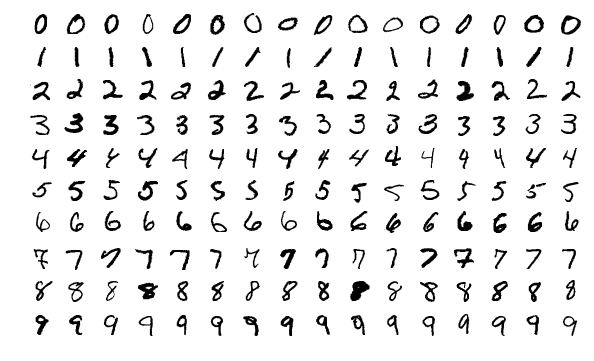
\includegraphics[width=\linewidth]{MnistExamples.png}
						\caption{Příklad obrázků z datasetu MNIST\\TODO(\url{https://upload.wikimedia.org/wikipedia/commons/2/27/MnistExamples.png})}
						\label{fig:MNIST}
					\end{figure}
					
					Tuto databázi jsem použil pro první testování BasicNeuralNetwork, jelikož má pro první testování dostačující velikost. Pro pozdější testování využívám převážně EMNIST.
				\subsection{Databáze EMNIST}
					\uv{Databáze MNIST se stala standardem pro učení umělého vidění. Databáze MNIST je odvozená z databáze NIST Special Database 19, která obsahuje ručně psané číslice a velká i malá písmena. EMNIST (Extended MNIST), varianta celé databáze NIST, přebírá uspořádání z databáze MNIST\footnote{Má však prohozené řádky a sloupce obrázků.}.} \parencite[přeloženo]{article:EMNIST}
					
					Tato databáze obsahuje více příkladů než MNIST, navíc obsahuje i sety s písmeny, proto jsem po prvních pokusech s MNIST přešel na tuto databázi.

		\chapter{Používání knihovny}


	\appendix
	\addcontentsline{toc}{part}{Apendix}
	
	\chapter*{Závěr}
	
		\lipsum[1]
	
	\nocite{*}
    \printbibliography					% Vytvoří seznam literatury
	\addcontentsline{toc}{chapter}{Bibliografie}
    \printglossary[title={Slovníček pojmů}]	% Vytvoří seznam zkratek
    \listoffigures						% Vytvoří seznam obrázků
    \listoftables						% Vytvoří seznam tabulek
    
    \begin{prilohy}
    	\pitem{Fotky z pokusů}
    	\eitem{Vlastní program}
    	\eitem{Dokumentace}
    	\eitem{Testovací data}
    \end{prilohy}
\end{document}